\documentclass[tikz]{standalone}

\usepackage{amssymb}
\usetikzlibrary{calc}
\usetikzlibrary{decorations.markings}
\begin{document}
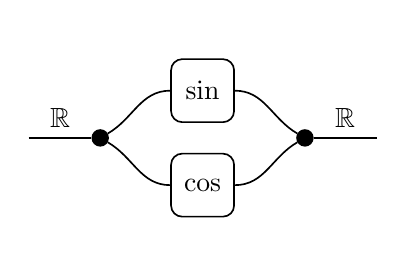
\begin{tikzpicture}[unit length/.code={{\newdimen\tikzunit}\setlength{\tikzunit}{#1}},unit length=4mm,x=\tikzunit,y=\tikzunit,semithick,box/.style={rectangle,draw,solid,rounded corners},junction/.style={circle,draw,fill,inner sep=0},outer box/.style={draw=none},wire/.style={draw,postaction={decorate},decoration={markings,mark=at position 0.5 with {\node[anchor=south] {#1};}}}]
\node[outer box,minimum width=11\tikzunit,minimum height=7\tikzunit] (root) at (0,0) {};\node[junction,minimum size=0.5\tikzunit] (n3) at (-3.25,0) {};\node[box,minimum size=2\tikzunit] (n4) at (0,1.5) {$\mathrm{sin}$};\node[box,minimum size=2\tikzunit] (n5) at (0,-1.5) {$\mathrm{cos}$};\node[junction,minimum size=0.5\tikzunit] (n6) at (3.25,0) {};\path[wire=$\mathbb{R}$] (root.west) to[out=0,in=180] (n3.180);\path[wire] (n3.30) to[out=30,in=-180] (n4.west);\path[wire] (n3.-30) to[out=-30,in=-180] (n5.west);\path[wire] (n4.east) to[out=0,in=150] (n6.150);\path[wire] (n5.east) to[out=0,in=-150] (n6.-150);\path[wire=$\mathbb{R}$] (n6.0) to[out=0,in=180] (root.east);
\end{tikzpicture}
\end{document}
